%\section{Android}

	\par Segundo \citeonline{monteiro2012}, Android é um sistema operacional
baseado em Linux, que utiliza a linguagem de programação Java para o
desenvolvimento de seus aplicativos. Criado especialmente para dispositivos
móveis, começou a ser desenvolvido no ano de 2003 pela então empresa Android
Inc, que em 2005 foi agregada ao Google. A partir de 2007 o projeto Android
uniu-se a Open Handset Alliance, uma associação de empresas de
softwares, hardwares e telecomunicações, que tem por finalidade desenvolver uma
plataforma para dispositivos móveis que seja completa, aberta e gratuita.

	\par \citeonline{krazit2009} afirma que o sistema pode rodar em equipamentos
de diversos fabricantes, evitando assim ficar limitado a poucos dispositivos.
Conforme informações do site \citeonline{android1}, hoje em dia existe mais de
um bilhão de aparelhos espalhados pelo mundo com esse sistema operacional.

	\par De acordo com \citeonline{monteiro2012}, as aplicações são executadas em
uma máquina virtual Java denominada Dalvik. Cada aplicativo, usa uma instância
dessa máquina virtual, tornando-o assim mais seguro. Por outro lado, os
softwares só podem acessar os recursos do dispositivo, como uma lista de
contatos, caso seja formalmente aceito pelo usuário nos termos de uso, ao
instalá-lo.

	\par As configurações de uma aplicação na plataforma Android ficam salvas em um
arquivo XML\footnote{XML - \textit{Extensible Markup Language}.} denominado
\texttt{AndroidManifest.xml}, que se localiza na pasta raiz do projeto. Para
\citeonline{lecheta2010}, as informações devem estar entre \textit{tags}
correspondentes ao recurso.

	\par \citeonline{lecheta2010} diz que as Intents são recursos tão importantes
que podem ser consideradas como o coração do Android e que estão presentes em
todas as aplicações.	De acordo com \citeonline[p.29]{k192012}, "Intents são
objetos responsáveis por passar informações, como se fossem mensagens, para os
principais componentes da API do Android, como as Activities, Services e
BroadCast Receivers". \citeonline{monteiro2012} diz que as Intents são criadas
quando se tem a intenção de realizar algo como por exemplo compartilhar uma
imagem, utilizando os app's já existentes no dispositivo. Existem dois tipos de
Intents:
	
	\begin{itemize}
	  
	  \item Intents implícitas: quando não é informada qual \textit{activity} deve
	  ser chamada, ficando assim por conta do sistema operacional verificar qual é a
	  melhor opção.
	  
	  \item Intents explícitas: quando é informada qual \textit{activity} deve ser chamada.
	  Usada normalmente para chamar \textit{activities} da mesma aplicação.
	  
	\end{itemize}
	
	\par Segundo \citeonline{k192012}, uma aplicação Android pode ser construída
com quatro tipos de componentes: Activity, Services, Content Providers e
Broadcast Receivers.

	\par As \textit{activities} são as telas com interface gráfica, que permitem
interações com os usuários. De acordo com \citeonline{lacheta2013}, cada
\textit{activity} tem um ciclo de vida, uma vez que ela pode estar sendo
executada, estar em segundo plano ou totalmente destruída.

	\par Toda vez que é iniciada uma \textit{activity}, ela vai para o topo de uma pilha
denominada \textit{activity stack}. O bom entendimento de seu ciclo de vida é
importante, pois quando uma aplicação é interrompida, é possível salvar as
informações ou ao menos voltar ao estágio a qual o usuário se encontrava. Na
Figura \ref{fig:qt1} é demonstrado o ciclo de vida de uma \textit{activity}.

	\begin{figure}[h!]
		\centerline{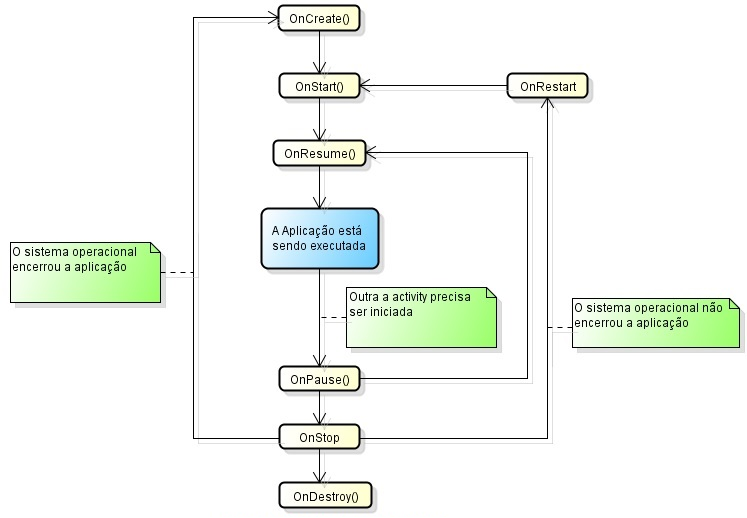
\includegraphics[scale=0.8]{./imagens/1_q_teorico/qt1.png}}
		\caption[Ciclo de Vida de uma activity]{Ciclo de Vida de uma
		\textit{activity}.
		 \textbf{Fonte:}\citeonline{lecheta2010}}
		\label{fig:qt1}
	\end{figure}

	\par Para que se possa entender melhor, imagina-se o seguinte cenário: um
usuário entra no aplicativo de notas da Univás. Para que a \textit{activity}
seja criada, é chamado o método \texttt{onCreate()}, logo após é executado o
método \texttt{onStart()} e ao finalizar do ciclo anterior é chamado o
\texttt{onResume()}, só a partir de então, a \textit{activity} é visualizada
pelo discente. Contudo, durante a navegação, o aluno recebe uma ligação, então
nessa hora o sistema operacional chama o método \texttt{onPause()} para
interromper a aplicação e abrir uma outra \textit{activity} para que o usuário
possa atender a chamada telefônica. É possível, nesse método, salvar
informações que o usuário está utilizando. Ao concluir o método de pausa, é
executado o método \texttt{onStop()}, a partir de agora a \textit{activity} da
Univás não será mais visível ao usuário.

 	\par Ao encerrar a ligação, há dois caminhos possíveis de se percorrer, o
primeiro, seria o caso do sistema operacional encerrar completamente a
aplicação, por necessidade de liberar espaço em memória. Para destrui-la é
chamado o método \texttt{onDestroy()}. Dessa forma, para executar o aplicativo
da Univás será necessário chamar o método \texttt{onCreate()} novamente
seguindo o ciclo normal. Porém se não for encerrada completamente, ao findar a
ligação será executado o método \texttt{onRestart()} e voltar para a
\textit{activity} ao qual o usuário se encontrava.

	\par No arquivo \texttt{AndroidManifest.xml} as \textit{activities} devem estar
entre as tags \texttt{<activity> </activity>} e a \textit{activity} principal,
ou seja, pela qual será iniciada a aplicação deve conter a \textit{tag}
\texttt{<intent-filter>} além de \texttt{<action
android:name="android.intent.action.MAIN"/>} indicando que essa atividade
deverá ser chamada ao iniciar a aplicação e \texttt{<category
android:\\name="android.intent.category.LAUNCHER"/>} que implica que esse
APP ficará disponível junto aos outros aplicativos no dispositivo.
Na figura \ref{fig:qt2} é apresentado o código do arquivo
\texttt{AndroidManifest.xml}. Nela, pode-se ver o nome da classe que será
iniciada e no atributo \textit{label} o nome que aparecerá na tela para o
usuário.
	
	\begin{figure}[h!]
		\begin{lstlisting}[style=custom_XML]
		  <activity
	            android:name=".MainActivity"
	            android:label="@string/app_name" >
	            <intent-filter>
	                <action android:name="android.intent.action.MAIN" />
	                <category android:name="android.intent.category.LAUNCHER" />
	            </intent-filter>
	      </activity>
		\end{lstlisting}
		\caption[Código do arquivo
		AndroidManifest.xml indicando qual activity deve ser executada quando a
		aplicação iniciar]{Código do arquivo \texttt{AndroidManifest.xml} indicando
		qual \textit{activity} deve ser executada quando a aplicação iniciar.
		 \textbf{Fonte:}Elaborado pelos autores}
		\label{fig:qt2}
	\end{figure}
	
	\par A \textit{activity} a ser utilizada para iniciar a aplicação é uma
\texttt{Navigation Drawer}, que segundo o site \citeonline{android2015}, ela exibe
do lado esquerdo as principais funções do software, semelhante a um
menu, que fica normalmente escondida aparecendo apenas quando clicado no canto
superior esquerdo. 

	\par Segundo \citeonline{lecheta2010}, a classe \texttt{Service} existe com o intuito
de executar processos que levarão um tempo indeterminado para serem executados
e que normalmente consomem um alto nível de memória e processamento. Esses
processos são executados em segundo plano enquanto o cliente realiza outra
tarefa. Assim um usuário pode navegar na internet enquanto é feito um
\textit{download}. O serviço é geralmente iniciado pelo \texttt{Broadcast Receiver} e
quem o gerencia é o sistema operacional que só o finalizará ao concluir a
tarefa, salvo quando o espaço em memória é insuficiente.

	\par Para \citeonline{lecheta2010}, um \texttt{Content Provider} provê conteúdos de
forma pública para todas as aplicações, possibilitando aos aplicativos consultar,
salvar, deletar e alterar informações no \textit{smartphone}. Assim afirma
\citeonline[p.413]{lecheta2010} “o Android tem uma série de provedores de
conteúdo nativos, como, por exemplo, consultar contatos da agenda, visualizar
os arquivos, imagens e vídeos disponíveis no celular”. Portanto, um contato
pode ser salvo na agenda de contatos do dispositivo por um aplicativo e
alterado por outro.

	\par Para \citeonline{monteiro2012}, o \texttt{Broadcast Receiver},
é um componente do Android responsável por responder a eventos do sistema.
Ele não possui interface gráfica e normalmente interage com os usuários através
de notificações.

	\par Outra ferramenta importante e muito utilizada do Android é a Notificação.
Segundo \citeonline{phillips2013} quando uma aplicação está sendo
executada em segundo plano e necessita comunicar-se com o usuário, o aplicativo
cria uma notificação. Normalmente as notificações aparecem na barra superior, o
qual pode ser acessado arrastando para baixo a partir da parte superior da
tela. Assim que o usuário clica na notificação ela cria uma \textit{activity}
para abrir  aplicação em questão.

	\par O Android traz embarcado em sua plataforma o banco de dados
\texttt{SQLite}, que armazena tabelas, \textit{views}, índices,
\textit{triggers} em apenas um arquivo em disco. Somente é possível acessa-lo
pela aplicação a qual o criou e, é deletado caso o aplicativo seja removido.

	\par Na seção abaixo serão descritos os elementos gráficos presentes no
Android.

	